\begin{figure}[h]
    \centering
    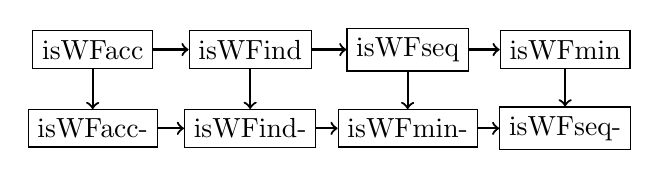
\begin{tikzpicture}[node distance=2cm, auto]
      % Standard definitions
      \node (std1) [draw] {isWFacc};
      \node (std2) [right of=std1, draw] {isWFind};
      \node (std3) [right of=std2, draw] {isWFseq};
      \node (std4) [right of=std3, draw] {isWFmin};
  
      % Weaker definitions
      \node (weak1) [below of=std1,  draw, yshift=1cm] {isWFacc-};
      \node (weak2) [below of=std2,  draw, yshift=1cm] {isWFind-};
      \node (weak3) [below of=std3,  draw, yshift=1cm] {isWFmin-};
      \node (weak4) [below of=std4,  draw, yshift=1cm] {isWFseq-};
  
      % Arrows
      \draw[->, thick] (std1) -- (weak1);
      \draw[->, thick] (std1) -- (std2);
      \draw[->, thick] (std2) -- (weak2);
      \draw[->, thick] (weak1) -- (weak2);
      \draw[->, thick] (std2) -- (std3) ;
      \draw[->, thick] (std3) -- (weak3);
      \draw[->, thick] (weak2) -- (weak3);
      \draw[->, thick] (std3) to (std4);
      \draw[->, thick] (weak3) to (weak4);
      \draw[->, thick] (std4) -- (weak4);
   \end{tikzpicture}
    % \caption{A graphic illustrating the implications we have found between the above
    % definitions and those we are still seeking to find. Green arrows indicate that one
    % definition implies another, red arrows indicate that we believe an implication should
    % be possible but we have not yet found it.
    % }
\end{figure}